% Chapter 17 -- English translation of chapters/c17.tex (French source): rusty-SUNDIALS, an AI-assisted Rust translation of the CVODE solver
% Figure: code/fig17.py.
\chapter[The calculation engine]{The calculation engine, and its inspection report}
\reference{Public repository created on 11 May 2026. Audit and retractions merged on 27 September 2026 (pull request no.~60). No DOI of its own.}

\noindent\niveau{X} for everything the solver computes: these are floating-point numbers; they guide and never
prove.

\section*{The idea in one picture}

\begin{analogie}
You are adjusting a shower whose water reacts quickly. The naive method is to look at the temperature \emph{now}
and turn the tap by that amount: if you turn too hard, the water goes from too hot to too cold, then to even
hotter, and the gap grows with every correction. The cautious method is to choose the tap position that will be
right \emph{once the correction has been made}. It takes a little calculation at each move, but it never runs
away. So-called ``stiff'' equations, in which some things change much faster than others, are showers of this
kind; the CVODE solver is built for them.

\emph{Where the picture stops:} a solver ``feels'' nothing, it solves an equation at each step; and the cautious
method stays stable without necessarily being accurate, as we see below.
\end{analogie}

\section*{What was done}

SUNDIALS is a widely used scientific computing library, written in the C language by a US national laboratory;
CVODE is the part that solves stiff equations from chemistry, plasmas or biology. From 11 May 2026, AI agents,
under the author's direction, made a translation of it into the Rust language, rusty-SUNDIALS. It became the
instrument of the year: the cosmological distances of Chapter~\ref{ch:c01}, the fixation probabilities of Chapter~\ref{ch:c06}, several
of the 25 October contributions and other papers rely on its calculations.

\paragraph{An example to follow with a pencil.} Take the equation $y'=-50\,y$ with $y(0)=1$, and a time step
$h=0.05$. The true solution is multiplied by $e^{-2.5}\approx0.082$ at each step: it dies out very quickly.
\begin{itemize}
\item The naive method (explicit Euler) computes $y_{n+1}=y_n+h\times(-50\,y_n)=(1-2.5)\,y_n=-1.5\,y_n$:
  $1$, then $-1.5$, then $2.25$, then $-3.375$\ldots{} It blows up while flipping sign, like the shower.
\item The cautious method (implicit Euler) imposes $y_{n+1}=y_n-2.5\,y_{n+1}$, hence $y_{n+1}=y_n/3.5$:
  $1$, $0.286$, $0.082$\ldots{} Less accurate than the true solution at each step, but always well behaved.
\end{itemize}
The naive one works only if $50\,h<2$, that is $h<0.04$. Figure~\ref{fig:c17} shows this threshold on a
neighbouring equation. This calculation was done in Python for this book: it illustrates the phenomenon, it is not
an output of rusty-SUNDIALS.

\section*{How we made sure it is not wrong}

Two things must be kept apart: the results of the papers that use the solver, and what the repository claimed about
itself.

For the autumn papers, auditors (AI agents distinct from the producers) reran the CVODE calculations and obtained
files identical byte for byte to the published ones. This proves that the calculation is reproducible, not that it
is correct; that is why these numbers stay at level~X and why the papers rely on them for no proven claim.

For the repository itself, the story is less flattering, and it matters just as much. On 27 September, three
separate AI agents audited its fusion work (the disruptions of the ITER reactor): one reread the claims of the
papers, another reran the calculations, a third checked the Lean files. Their findings:
\begin{itemize}
\item published numbers were produced by no code in the repository; they were values typed by hand;
\item a program printed ``47-fold speed-up mathematically verified''; without the pauses (\texttt{sleep})
  inserted into the code, the ratio of the two times was $1.00$;
\item the plot of a formula fixed in advance was passed off as a plasma ``simulation'';
\item Lean ``certificates'' were empty, or rested on axioms from which falsehood can be deduced, which the audit
  demonstrated in the kernel itself.
\end{itemize}
A retraction notice was merged the same day. Nothing was erased: every document carries a banner pointing to the
notice, and the code that used to print invented verdicts now prints what it measures, or ``NOT MEASURED''. On its
own control tests, the audit found the solver correct at moderate tolerances, and noted that a stiffer case fails
at a very fine tolerance. No human has reviewed these audits.

\section*{What this does not say}

\begin{limite}
\begin{itemize}
\item The solver is not ``formally verified'', despite what the front page of its repository still announces.
  Its outputs are floating-point calculations (\niveau{X}).
\item Several Lean specification files in the repository contain empty or inconsistent axioms; nothing should be
  built on them.
\item As of 26 October 2026, the repository's metadata sheet still repeats retracted claims; the audit left this
  choice to the owner, and it has not been made.
\item A file identical byte for byte shows that the calculation can be redone, not that it is exact.
\item The audit noted a difference from the original in how the solver reacts to repeated failures of its error
  test; it flags this as a hypothesis, not verified.
\end{itemize}
\end{limite}

\section*{Going further}

The public repository rusty-SUNDIALS contains the code, and the folder of the 27 September audit (retraction
notice and three reports). Chapter~\ref{ch:c20} tells of another numerical method wrongly accused, then measured.

\begin{figure}[t]
\centering
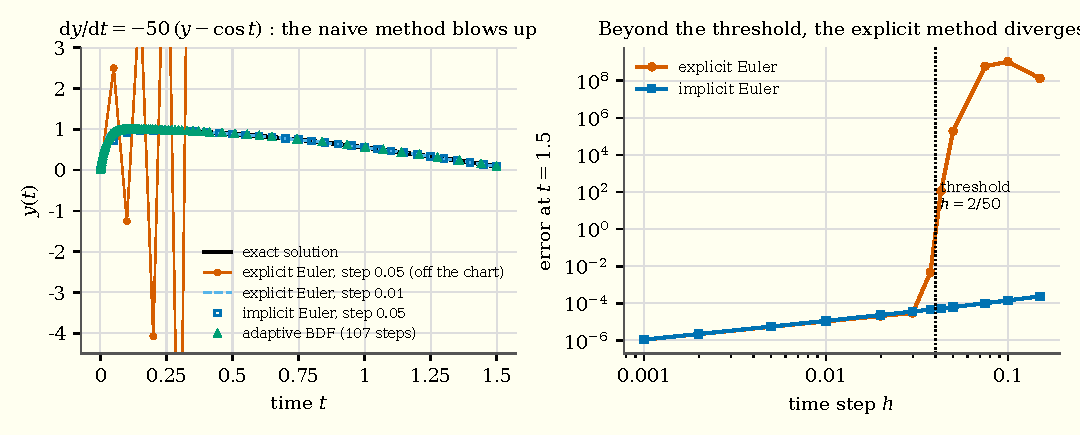
\includegraphics[width=\linewidth]{figures/c17_raideur}
\caption{Illustrative calculation in Python (not rusty-SUNDIALS). Left: the stiff equation $y'=-50(y-\cos t)$; the
naive method with step $0.05$ blows up, the others follow the exact solution. Right: final error as a function of
the step; the naive method diverges beyond $h=2/50$.}
\label{fig:c17}
\end{figure}
